\section{Definition av skärningstalet}\par
\noindent "tredje halvan" av kursen. Från början formulerade vi Bezouts pseudosats som inte var sann, men för att göra den sann tittade vi på komplexa projektiva världen och införa skärningstalet och visa Bezouts sats. Sedan har vi använt Bezouts sats för att räkna singulära punkter på kurvor, vi har tittat på kurvor givet 5 punkter, vi har tittat på elliptiska kurvor och allmänna tredjegradskurvor
\par\bigskip
\noindent Vi har gjort allt nogrannt, men vi har inte definierat skärningstalet (enbart axiomatiskt).\par
\noindent Skärningstalsfunktionen är unik i sin existens, detta går även att räkna fram ur axiomen.\par
\noindent Vad vi vill göra är att ha en konstruktion för skärningstalet, så att vi vet att det existerar och inte bara är unikt. För att komma dit, ska vi ta en väg via klasser av funktioner på kurvor och liknande samt generalisera av det vi gjort hittils (till enklare fall), samt Hillberts nollställessats
\par\bigskip
\noindent Vi behöver vissa algebraiska verktyg:\par
\begin{itemize}
  \item Ringar
  \item Ideal
  \item Kvotringar
  \item + lite till 
\end{itemize}
\par\bigskip
\subsection{Generalisering}\hfill\\\par
\begin{theo}[Affin algebraisk mängd]{thm:affinalgset}
  En \textit{affin algebraisk mängd} $X\subseteq \C^n$ är en mängd på formen:
  \begin{equation*}
    \begin{gathered}
      X = V(F) = \left\{\overline{x}\in\C^n\:|\: f(\overline{x}=0\quad\forall f\in F)\right\}\qquad F\subseteq\C[x_1,\cdots,x_n]
    \end{gathered}
  \end{equation*}\par
  \noindent Beteckna med $(F)$ idealet som genereras av $F$\par
  \noindent Det är lätt att se att $V(F) = V((F))$, så algebraiska mängder hör ihop med ideal på något sätt, likt hur i linjär algebra kunde vi använda gausseliminering utan att ändra lösningsmängden (trots att vi ändrar ekvationssystemen)
\end{theo}
\par\bigskip
\begin{theo}[Hillberts bassats]{thm:hilnrewirg}
  Varje ideal i $\C[x_1,\cdots,x_n]$ är \textit{ändligt genererat}!
  \begin{equation*}
    \begin{gathered}
      I =(f_1,\cdots,f_n)\subseteq\C[x_1,\cdots,x_n]
    \end{gathered}
  \end{equation*}\par
  \noindent Vi studerar bara ändliga ekvationssystem, men kan ändå säga saker om oändligheten
\end{theo}
\par\bigskip
\noindent Nu har vi alltså någon relation som tar ett ideal och ger en algebraisk mängd:
\begin{equation*}
  \begin{gathered}
    \left\{\text{ideal}\right\}\to\left\{\text{algebraisk mängd}\right\}\\
    I\to V(I)
  \end{gathered}
\end{equation*}\par
\noindent Vi visar andra riktningen. Givet en algebraisk mängd $X\subseteq \C^n$, så sätter vi säg $I(X)$ som:
\begin{equation*}
  \begin{gathered}
    I(X) = \left\{f\in\C[x_1,\cdots,x_n]\:|\: f|_X=0\right\}\subseteq\C[x_1,\cdots,x_n]
  \end{gathered}
\end{equation*}\par
\noindent Detta är ett ideal, vi ser att vi får:
\begin{equation*}
  \begin{gathered}
    X\to I(X)
  \end{gathered}
\end{equation*}\par
\noindent Detta ser nästan ut som en bijektion, men vi måste vara lite petigare.
\begin{equation*}
  \begin{gathered}
    V(I(X)) = X
  \end{gathered}
\end{equation*}\par
\noindent Motsvarande gällar \textit{nästan}:
\begin{equation*}
  \begin{gathered}
    I\subseteq I(V(I))
  \end{gathered}
\end{equation*}\par
\noindent Det omvända gäller ej i allmänhet:
\begin{equation*}
  \begin{gathered}
    I(V(I))\subseteq I
  \end{gathered}
\end{equation*}
\par\bigskip
\noindent\textbf{Exempel:}\par
\noindent Låt $n=1$ och titta på idealet som genereras av polymomet $x^2$:
\begin{equation*}
  \begin{gathered}
    I = (x^2)\subseteq\C[x]\\
    V(I) = \left\{0\right\}\subseteq \C\\
    I(\left\{0\right\}) = (x)
  \end{gathered}
\end{equation*}\par
\noindent Notera, alla rötter till element i $(x^2)$ ligger inte i $(x^2)$ 
\par\bigskip
\begin{theo}[Hillberts nollställessats]{thm:hillbertnulls}
  Korrespondensen som vi har skisserat ger en bijektion:
  \begin{equation*}
    \begin{gathered}
      \left\{\text{radikalideal i $\C[x_1,\cdots,x_n]$}\right\}\stackrel{\approx}{\leftrightarrow}\left\{\text{algebraiska mängder i }\C^n\right\}
    \end{gathered}
  \end{equation*}
\end{theo}
\par\bigskip
\noindent Vi har inte sagt vad radikalideal ideal är, men det kommer visa sig att alla primideal är radikalideal, och från algebra 2 vet vi att maximala ideal är primideal.\par
\noindent Maximala ideal kommer motsvara så små algebraiska mängder som möjligt, de motsvarar enstakta punkter\par
\noindent Primideal motsvarar irreducibla algebraiska mängder (sådana som bara är en bit)\par
\noindent Radikala ideal motsvarar mer allmänna saker.
\par\bigskip
\noindent Låt $R$ vara en kommutativ ring, och $I\subseteq R$ är ett ideal
\par\bigskip
\begin{theo}[Primideal]{thm:primeideal}
  $I$ kallas ett \textit{primideal} om $R\backslash I$ är en "multiplikativ mängd", dvs:
  \begin{equation*}
    \begin{gathered}
      1\notin I\backslash\\
      f,g\notin I\Rightarrow fg\notin I
    \end{gathered}
  \end{equation*}\par
  \noindent Om $R\backslash I$ och $I$ primideal, så är kvotringen ett integritetsområde 
\end{theo}
\par\bigskip
\begin{theo}[Maximal ideal]{thm:maxideal}
  $I$ kallas för ett maximalt ideal om:
  \begin{equation*}
    \begin{gathered}
      I\subsetneq J\Rightarrow J=R
    \end{gathered}
  \end{equation*}
\end{theo}
\par\bigskip
\begin{theo}[Kvotringen]{thm:quotientring}
  Man inför $\sim$ på $R$ som ges av att:
  \begin{equation*}
    \begin{gathered}
      x\sim y\Lrarr x-y\in I
    \end{gathered}
  \end{equation*}\par
  \noindent Här är $R\backslash I$ en kropp
\end{theo}
\par\bigskip
\begin{theo}[Radikalen till ideal]{thm:radicalidear}
  Betecknas med $\sqrt{I}$ och är:
  \begin{equation*}
    \begin{gathered}
    \sqrt{I} = \left\{x\in R\:|\:\exists m\in\N\:|\: x^m\in I\right\}
    \end{gathered}
  \end{equation*}
\end{theo}
\par\bigskip
\noindent\textbf{Notera:}\par
\noindent Radikalen innehåller i (sätt $m=1$ så får du $I$), och radikalen är ett ideal
\par\bigskip
\begin{theo}{Radikalideal}{thm:radicalideal}
  Ett \textit{radikalideal} är ett ideal $I$ så att $I = \sqrt{I}$
\end{theo}
\par\bigskip
\noindent\textbf{Exempel:}\par
\noindent Betrakta $4\Z\subseteq\Z$, vi hävdar att detta inte är ett radikalideal ty $2^2\in4\Z$ men $2\notin4\Z$
\par\bigskip
\noindent\textbf{Exempel:}\par
\noindent $6\Z\subseteq\Z$ är ett radikalideal:
\begin{equation*}
  \begin{gathered}
    x^m = 2\cdot3\cdot n\Rightarrow 2|x\;3|x\Rightarrow 6|x
  \end{gathered}
\end{equation*}
\par\bigskip
\begin{theo}
  VVarje primideal är radikalt
\end{theo}
\par\bigskip
\begin{prf}
  FFöljer direkt från definition. Låt $p$ vara primideal:
  \begin{equation*}
    \begin{gathered}
      x\notin p\Rightarrow x^m\notin p\quad\forall m
    \end{gathered}
  \end{equation*}
\end{prf}
\par\bigskip
\noindent\textbf{Exempel:}\par
\noindent $(x^2)$ är \textit{inte} radikalt i $\C[x]$ ty $\sqrt{(x^2)} = (x)$
\par\bigskip
\begin{theo}
  A$I\subseteq R$ är radikalideal $\Lrarr R/I$ saknar nollskillda nilpotenta element
\end{theo}
\par\bigskip
\begin{theo}[Nilpotent]{thm:nilpotent}
  $x$ är nilpotent om $\exists m\in\N$ så att $x^m=0\Lrarr R/I$ är reducerad 
\end{theo}
\par\bigskip
\noindent Låt $I\subseteq\C[x_1,\cdots,x_n]$ vara ett radikalideal och $V(I)$ motsvarande algebraiska mängd.
\par\bigskip
\begin{theo}[Koordinatringen]{thm:coordinatering}
  $V$:s \textit{koordinatring} eller \textit{ringen av reguljära funktioner} definieras som:
  \begin{equation*}
    \begin{gathered}
      \C[V] = \C[x_1,\cdots,x_n]/I\qquad\C[\C^n] = \C[x_1,\cdots,x_n]\\
      =\left\{\text{polynomfunktioner $f,g$ där $f=g\Lrarr f|_V=g|_V$}\right\}
    \end{gathered}
  \end{equation*}
\end{theo}
\par\bigskip
\noindent\textbf{Exempel:}\par
\noindent I dimension 2, tag $V=x$-axeln, alltså $V = \left\{y=0\right\} = V(y)$.\par
\noindent Koordinatringen är då $\C[x,y]/(y) \cong\C[x]$\par
\noindent Vad vi vet om denna kvotring är att den saknar nilpotenta element. Detta är naturligt om vi tänker på det som en funktion av komplexa värden. \par
\noindent $V$ är en irreducibel algebraisk mängd, kvotringen är ett integritetsområde.
\par\bigskip
\noindent\textbf{Exempel:}\par
\noindent $V = \left\{(a_1,b_1),\cdots,(a_m,b_m)\right\}\subseteq\C^2$, då är $I(\left\{(a_i,b_i)\right\}) = (x-a_i,y-b_i)$ maximalt ideal $\Lrarr (a_i,b_i)$.\par
\begin{equation*}
  \begin{gathered}
    I(V) = \bigcap_{i}(x-a_i,y_bi)\\
    \C[x,y]\to\C^m\\
    f\to (f(a_1,b_1),\cdots,f(a_n,b_n))
  \end{gathered}
\end{equation*}\par
\noindent Det visar sig att detta ger en relation mellan algebraiska mängder och reducerade ändligt genererade $\C$-algebror:
\begin{equation*}
  \begin{gathered}
    X\to\C[X]
  \end{gathered}
\end{equation*}
\par\bigskip
\noindent\textbf{Anmärkning:}\par
\noindent Om $V$ är irreducibel så är $I(V)$ primideal, så $\C[V]$ har inga 0-delare
\par\bigskip
\noindent\textbf{Exempel:}\par
\noindent Betrakta $f(x,y)=xy=0$, då är $\C[V]/(xy)$ \textit{inte} ett integritetsområde (det finns nolldelare, nämligen $x$ och $y$)
\begin{equation*}
  \begin{gathered}
    \begin{rcases}
      x+(xy)\neq0\\
      y+(xy)\neq0
    \end{rcases}\text{ är nolldelare}
  \end{gathered}
\end{equation*}
\par\bigskip
\noindent\textbf{Kuriosa:}\par
\noindent Koordinatringen heter så för den genereras av $x$ och $y$
\par\bigskip
\noindent\textbf{Anti-Exempel:}\par
\noindent Ett exempel på något som \textit{nästan} är en koordinatring, men som inte är det:
\begin{equation*}
  \begin{gathered}
    \C[x]/(x^2)
  \end{gathered}
\end{equation*}\par
\noindent är inte en koordinatring, men "ser ut" som en. Problemet är att $(x^2)$ är inte ett radikalideal.\par
\noindent Det kommer att visa sig att vi ändå kommer vara intresserade att studera denna ring, ty vi vill studera "dubbelpunkten 0" (punkten 0 med multiplictet 0).
\par\bigskip
\begin{theo}
  ELåt $V\subset\C^m$. En reguljär avbildning $\overline{f}:V\to\C^m$ är en avbildning som ges av polynomiela funktioner ($m$st polynom i variablerna $x_1,\cdots,x_n$)
  \par\bigskip
  \noindent Har reguljära komponentfunktioner, med andra ord, $\overline{f}$ är restriktionen av någon\par
  $\C^n\to\C^m$ $(x_1,\cdots,x_n)\mapsto(f_1(\overline{x}),\cdots,f_m(\overline{x}))$
\end{theo}
\par\bigskip
\noindent\textbf{Anmärkning:}\par
\noindent Polynomfunktioner på $V$ kallas fö \textit{reguljära} funktioner. Alternativt "polynomiella avbildningar"
\par\bigskip
\noindent\textbf{Exempel:}\par
\noindent En avbildning vi är väldigt bekant med är affina avbildningar. Ett annat exempel är följande:
\begin{equation*}
  \begin{gathered}
    p(x)\in\C[x]\\
    g:\C\to\C^2\qquad x\mapsto(x,p(x))\qquad\text{(parametrisering av grafen till $p$)}
  \end{gathered}
\end{equation*}\par
\noindent Detta är en reguljär avbildning, $p$ är polynom.\par
\noindent Bilden av grafen är $g(\C) = \Gamma\subset\C^2$
\par\bigskip
\noindent\textbf{Exempel:}\par
\noindent Projektionen $\pi:\C^2\to\C$ så att $(x,y)\mapsto x$ är också reguljär, $x$ är polynom.
\par\bigskip
\noindent Vi kan sammansätta våra exempel:
\begin{equation*}
  \begin{gathered}
    \pi\circ g(x) = id_\C(x) = x\\
    g\circ \pi|_\Gamma(x,p(x)) = (x,p(x))
  \end{gathered}
\end{equation*}
\newpage
\noindent Mer intuitivt:
\begin{figure}[ht!]
    \centering
    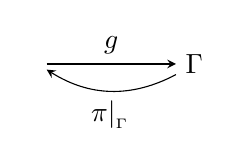
\begin{tikzpicture}
      \node[](p0){$\C$};
      \node[right of=p0, xshift=1cm](p1){$\Gamma$};
      \path[-stealth] (p0) edge[above] node{$g$} (p1);
      \path[-stealth] (p1) edge[below,bend left] node{$\pi|_{_\Gamma}$} (p0);
    \end{tikzpicture}
    \caption{$\C$ och $\Gamma$ är isomorfa}
\end{figure}
\par\bigskip
%\noindent\textbf{Anmärkning:}\par
%\noindent Affina avbildningar får inte ändra grad
\par\bigskip
\noindent\textbf{Exempel:}\par
\noindent $y^2=x^3$ är klassiskt exempel. Kalla den för $V$\par
\noindent Betrakta nu:
\begin{equation*}
  \begin{gathered}
    f:\C\to\C^2\\
    t\mapsto (t^2,t^3)
  \end{gathered}
\end{equation*}\\
\noindent Här är $f(\C) = V$, men! Inversen till denna avbildning är
\begin{equation*}
  \begin{gathered}\\
    \dfrac{t^3}{t^2} = t
    (x,y)\mapsto \dfrac{y}{x}
  \end{gathered}
\end{equation*}\par
\noindent Men denna är inte definierad i 0, så det är ingen reguljär avbildning. Det finns ingen reguljär invers. Då är kurvorna \textit{inte} isomorfa. Detta beror på att $V$ har en singuläritet i origo. 
\par\bigskip
\subsection{Rationella fukntioner}\hfill\\\par
\noindent Notera, fraktionskropp är bråkkropp och betecknas $Q(R)$ för en ring $R$
\par\bigskip
\noindent Om $V\subseteq\C^n$ är irreducibel så är $I(V)$ primideal och $\C[V]$ är därför ett integritetsområde och har därför en bråkkropp som kallas för $\C(v)$ (ringen av rationella funktioner, kallas ävne för funktionskropp)
\par\bigskip
\noindent\textbf{Anmärkning:}\par
\noindent Rationella funktioner är inte riktigt funktioner (de är inte definierade överallt). Tänk på de som funktioner som har vissa problem. De är väldit väldigt nära att bli funktioner dock! 
\par\bigskip
\noindent\textbf{Anmärkning:}\par
\noindent En rationell funktion kallas \textit{reguljär} i punkten $p$ om den kan skrivas på följande:
\begin{equation*}
  \begin{gathered}
    f = \dfrac{g}{h}\qquad\text{$h(p)\neq0$}
  \end{gathered}
\end{equation*}
\par\bigskip
\noindent En rationell avbildning är en som ges av rationella funktioner i varje "lucka". En flervariabelvariant/vektorvärd variant av rationella funktioner.
\par\bigskip
\noindent\textbf{Exempel:}\par
\noindent Det första exemplet är exemplet med avbildningen $t\mapsto (t^2,t^3)$, även det omvända, dvs $(x,y)\mapsto\dfrac{x}{y}$ är rationell, men den har problem, men den är fortfarande en rationell avbildning.
\par\bigskip
\noindent Exemplet med $y^2=x^3$ är inte isomorf med $\C$, men de är \textit{birationell ekvivalenta}.
\par\bigskip
\noindent Rationella avbildningar är bra när man vill studera singuläriteter eller även projektiva avbildningar.\par
\noindent Projektiva avbildningar ges av linjära avbildningar från $\C^3\to\C^3$:
\begin{equation*}
  \begin{gathered}
    (x,y,z)\mapsto(ax+by+cz,dx+ey+fz,gx+hy+kz)
  \end{gathered}
\end{equation*}\par
\noindent Här ser den väldigt reguljär ut, så vi betraktar den i en karta, säg $xy$-kartan:
\begin{equation*}
  \begin{gathered}
    (x,y,z)\mapsto\left(\dfrac{ax+by+c}{gx+hy+k},\dfrac{dx+ey+f}{gx+hy+k}\right)
  \end{gathered}
\end{equation*}
\par\bigskip
\subsection{Sammanfattning}\hfill\\\par
\noindent Reguljära funktioner: $\C[V]$-koordinatringen \par
\noindent Rationella funktioner: $\C(V)$-funktionskroppen\par
\noindent Reguljära avbildningar: Viktigaste exemplet är affina transformationer\par
\noindent Rationella avbildningar: Viktigaste exemplet är projektiva transformationer
